% Chapter 5

\chapter{Symmetries, topology and edge states } % Main chapter title

\label{Chapter5} % For referencing the chapter elsewhere, use \ref{Chapter5} 

\lhead{Part II. \emph{Kitaev wires}}
\chead{Chapter 5. \emph{Symmetries, topology \& edge states}} % This is for the header on each page - perhaps a shortened title

%----------------------------------------------------------------------------------------
In this chapter we study the symmetries and topology of the Kitaev wires. In section \ref{sec.SymmetriesTRandPH} we define the time reversal, particle-hole and sublattice transformations. We further show, that the system has an intrinsic particle-hole symmetry. In section \ref{sec.Topology10foldway} we use the transformations to formulate the topological classification dubbed the tenfold way. In section \ref{sec.2wirestimereversalsymmetries} we analyse the time reversal symmetries of the system. In turn the system is classified according to the tenfold way. In section \ref{sec.2wires_CSinv} we calculate the topological invariants of the system. In section \ref{sec.separatedwires} we study the separated wires and show that these support edge states. In section \ref{sec.2wireskramersdegeneracy} we study how the interwire interaction affects the edge states. Finally, in section \ref{sec.2wirestransitionqualitative} we formulate two possibilities for the $p$- to $s$-wave phase transition in a qualitative manner. 


\section{Time reversal, particle-hole and sublattice transformations}
\label{sec.SymmetriesTRandPH}
The mean field Hamiltonian is diagonal in momentum space. This means, that it is translationally invariant. Specifically, the (unitary) translation operator is defined through: $\tau(x_0)\psi_{j,F}(x)\tau^\dagger (x_0) = \psi_{j,F}(x + x_0)$. In momentum space, we hereby get $\tau(x_0) c_{j,k} \tau^\dagger(x_0) = \text{e}^{ikx_0}c_{j,k}$, as one might expect. Hence, terms like $c^\dagger_{j,k} c_{j,k}$ and $c_{i,k}c_{j,-k}$ are invariant under the translation. This means, that $H_{FF}$ is invariant as well. Because of the translational invariance, we \textit{inforce} that the time reversal, $T$, and particle-hole transformation, $C$, do not mix states with different positions. Specifically:
\begin{align}
T \Psi(x) T^{-1} &= U^\dagger_T \Psi(x), \hspace{0.5cm} TiT^{-1} = -i, \nonumber \\
C \Psi(x) C^{-1} &= (U^*_C)^\dagger (\Psi^\dagger(x))^t, \hspace{0.5cm} CiC^{-1} = i, 
\label{eq.TRandPH.realspace}
\end{align}
with $\Psi(x) = \begin{bmatrix} \psi_{1,F}(x) & \psi^\dagger_{1,F}(x) & \psi_{2,F}(x) & \psi^\dagger_{2,F}(x) \end{bmatrix}^t$, $t$ the transpose operation and $T$, $C$ the time reversal and particle-hole transformation respectively. The construction $(\Psi^\dagger(x))^t$ is to make the entries of $\Psi(x)$ daggered, but still have $\Psi(x)$ as a column vector. The trivial particle-hole transformation, i.e. $U_C = \mathbb{I}$, is hereby $\psi_{j,F}(x) \to \psi^\dagger_{j,F}(x)$. $U_T$ and $U_C$ are $4\times 4$ matrices. Inforcing that the transformed operators are fermionic as well ensures these matrices to be unitary. The operation on $i$ specifies, that time reversal is antiunitary and the particle-hole transformation is unitary. In momentum space this definition leads to:
\begin{equation}
T C_k T^{-1} = U^\dagger_T C_{-k}, \hspace{0.5cm} C C_k C^{-1} = (U^*_C)^\dagger (C^\dagger_{-k})^t,  
\label{eq.TRandPH.momentumspace}
\end{equation}
with $C_k = \begin{bmatrix} c_{1,k} & c^\dagger_{1,-k} & c_{2,k} & c^\dagger_{2,-k} \end{bmatrix}^t$. In momentum space, the trivial particle-hole transformation is $c_{j,k} \to c^\dagger_{j,-k}$. By inspecting the transformations $TH_{FF}T^{-1}$ and $CH_{FF}C^{-1}$, we get the following symmetry requirements:
\begin{align}
TH_{FF}T^{-1} = H_{FF} \Leftrightarrow U_T\mathcal{H}^*_{FF,-k} U^\dagger_T = + \mathcal{H}_{FF,+k}, \nonumber \\
CH_{FF}T^{-1} = H_{FF} \Leftrightarrow U_C\mathcal{H}^*_{FF,-k} U^\dagger_C = - \mathcal{H}_{FF,+k}. 
\label{eq.Symmetryrequirements}
\end{align}
This means, that we can think of the second quantization transformations $T$ and $C$ in terms of first quantization antiunitary transformations $\mathcal{T} = U_TK$ and $\mathcal{C} = U_CK$, where $K$ is the complex conjugation operator. This is a general property of these transformation, not restricted to our specific system. See e.g. the articles \cite{Ludwig.Topology, Chiu.Topology}. The Hamiltonian at hand is a socalled Bogoliubov-de Gennes (BdG) Hamiltonian. These BdG Hamiltonians in general have a particle-hole symmetry. The reason is, that there is a redundancy in the matrix structure of the Hamiltonian. Explicitly, the structure contains a $4\times 4$ matrix, even though there are only two energy solutions for each $k$. Another way of putting this is that the two Nambu spinors, $C^\dagger_k$ and $C_k$ are not independent. We can transform one into the other by going to $-k$ and flipping the entries. The redundancy is here especially evident, since we can simply choose $C$ to have no effect on the Nambu spinor:
\begin{equation}
C C_k C^{-1} =  \sigma_0\otimes \tau_1 (C^\dagger_{-k})^t = \begin{bmatrix} 0 & 1 & 0 & 0 \\ 1 & 0 & 0 & 0 \\ 0 & 0 & 0 & 1 \\ 0 & 0 & 1 & 0 \end{bmatrix} \begin{bmatrix} c^\dagger_{1,-k} \\ c_{1,k} \\ c^\dagger_{2,-k} \\ c_{2,k} \end{bmatrix} = \begin{bmatrix} c_{1,k} \\ c^\dagger_{1,-k} \\ c_{2,k} \\ c^\dagger_{2,-k} \end{bmatrix} = C_k,
\end{equation}
with $\sigma_0$ the identity in wire space and $\tau_1$ the first Pauli matrix in particle-hole space. $\otimes$ is the direct matrix product. This means, that $H_{FF}$ is invariant under $C$. Since it stems from a redundancy in the \textit{structure} of the Hamiltonian, it is often referred to as a particle-hole \textit{constraint} of BdG systems rather than a symmetry. This also means that for the system to be consistent, we need $(\sigma_0\otimes\tau_1)\mathcal{H}^*_{FF,+k}(\sigma_0\otimes\tau_1) = - \mathcal{H}_{FF,-k}$, which can also explicitly be checked. 

By composing the time reversal and particle-hole transformations we can form a third transformation; the sublattice (or chiral) transformation $S = TC$. It is evident, that this transformation is antiunitary like $T$. The same analysis as in the above leads to the symmetry condition:
\begin{equation}
SH_{FF}S^{-1} = H_{FF} \Leftrightarrow U_S\mathcal{H}_{FF,+k} U^\dagger_S = - \mathcal{H}_{FF,+k}.
\end{equation}
Hence, the transformation in first quantization is unitary, but has to anticommute with the Hamiltonian. We explain the reason for studying these transformations in the next section.

\section{Topology and the tenfold way} \label{sec.Topology10foldway}
In the articles \cite{Ludwig.Topology, Chiu.Topology} it is studied, how one in the broadest possible sense can classify \textit{all} noninteracting fermionic Hamiltonians, that has an energy gap in the spectrum. This includes insulators and superconductors. Hence, the authors build a framework in which two distinct Hamiltonians are viewed as equivalent, if one can continuously deform one to the other without closing the energy gap. These sort of deformations are linked to the study of topological spaces, also called manifolds. Hence, the term \textit{topology}. Later we will see, that the topology of the Hamiltonian has geometrical effects in real space, the edge states. However, as the above makes it clear, this is not the source of the term topology.  

One can use the three transformations of the previous section to classify the system within the above framework in the following manner. There are three possibilities for the time reversal and particle-hole symmetries. Either there is no symmetry, indicated by a $0$, or there is a symmetry and then the transformations can square to plus and minus the identity, indicated with $\pm 1$. The sublattice symmetry can either by absent, $0$, or present, $1$. Per construction, if there is both a time reversal, $T$, and a particle-hole symmetry, $C$, present, there is also a sublattice symmetry, $S=TC$. On the other hand, if only $T$ or $C$ is present of the two, there cannot be a sublattice symmetry. Else, we would be able to make the remaining symmetry by composition. However, in the case of no $T$ nor $C$ symmetry, there is still two possibilities for $S$: symmetry or no symmetry. This is the reason why this last transformation is included. In total we then have $(3\cdot 3 - 1) + 2 = 10$ possibilities of combining the symmetries. It is therefore also referred to as the tenfold way. 

\begin{table}[htb]
\centering
\caption{\textit{Periodic table of topological superconductors and insulators. $d$ is the spatial dimension. A 0-value for T,C and S indicates no symmetry. For T and C the sign indicates the sign of the square $T^2$ and $C^2$ for a symmetry present. $S=1$ indicates presence of a sublattice symmetry. The sets to the right indicates in what set of numbers the topological index should be found. }}
\begin{tabular}{|l||l l l||l l l l|}
\hline Cartan/$d$   &  T &  C & S					& 0 & 1 & 2 & 3 \\ \hline 
\hline A    		&  0 &  0 & 0					& $\mathbb{Z}$ & 0 & $\mathbb{Z}$ & 0   			 \\
\hline AIII 		&  0 &  0 & 1					& 0 & $\mathbb{Z}$ & 0 & $\mathbb{Z}$   			 \\
\hline AI   		& +1 &  0 & 0					& $\mathbb{Z}$ & 0 & 0 & 0 			    			 \\
\hline BDI	       	& +1 & +1 & 1 					& $\mathbb{Z}_2$ & $\mathbb{Z}$ & 0 & 0 			 \\
\hline D	       	&  0 & +1 & 0 					& $\mathbb{Z}_2$ & $\mathbb{Z}_2$ & $\mathbb{Z}$ & 0 \\
\hline DIII	       	& -1 & +1 & 1 					& 0 & $\mathbb{Z}_2$ & $\mathbb{Z}_2$ & $\mathbb{Z}$ \\
\hline AII	       	& -1 &  0 & 0 				 	& $2\mathbb{Z}$ & 0 & $\mathbb{Z}_2$ & $\mathbb{Z}$  \\
\hline CII	       	& -1 & -1 & 1 					& 0 & $2\mathbb{Z}$ & 0 & $\mathbb{Z}_2$  			 \\
\hline C	       	&  0 & -1 & 0 					& 0 & 0 & $2\mathbb{Z}$ & 0  						 \\
\hline CI	       	& +1 & -1 & 1 					& 0 & 0 & 0 & $2\mathbb{Z}$  						 \\
\hline 
\end{tabular}
\label{tab.PeriodicTableTISC}
\end{table}

Classifying the Hamiltonians in this framework puts the Hamiltonian in a specific Cartan class. The information from the classification is, that the socalled topological index has to be found in a specific set of numbers. This set can for example be the integers, $\mathbb{Z}$. The result of the articles is then, that if two ground states have different integers as their topological index, they cannot be deformed continously into each other. This means, that the deformation from one to the other includes a closing of the energy gap. The socalled periodic table for topological insulators and superconductors is shown in table \ref{tab.PeriodicTableTISC}.


\section{Time reversal symmetries} \label{sec.2wirestimereversalsymmetries}

\subsection{With wire exchange}
\label{subsec.TRwireexchange}
In this subsection we will show, that we can construct two types of time reversal symmetries of the system, that exchange the wires. One is obeyed if the interwire pairing is imaginary; this squares to $+\mathbb{I}$. The other is obeyed if the interwire pairing is real; this squares to $-\mathbb{I}$. We will further shortly discuss the particle-hole and sublattice symmetries, and finally how these symmetries puts the Hamiltonian in a specific symmetry class. 

We first define a time reversal operator, that squares to $ + \mathbb{I}$ and interchanges the wires: 
\begin{equation}
T_+\begin{bmatrix} c^\dagger_{1,k} \\ c^\dagger_{2,k} \end{bmatrix} T_+^{-1} = \eta\sigma_1 \begin{bmatrix} c^\dagger_{1,-k} \\ c^\dagger_{2,-k} \end{bmatrix} = \eta\begin{bmatrix} c^\dagger_{2,-k} \\ c^\dagger_{1,-k} \end{bmatrix},\nonumber
\end{equation} 
with $\sigma_1$ the first Pauli matrix operating in wire space and $\eta$ some overall phase. Hence, under this time reversal transformation a fermion from wire 1 is transformed into a fermion in wire 2 and acquires the phase $\eta$. Since $(\eta\sigma_1)(\eta\sigma_1)^* = \sigma_1^2 = + \mathbb{I}$ we get, that $T_+$ squares to plus the identity. The question is now: under what circumstances is $T_+$ a symmetry of the Hamiltonian? Since $\varepsilon_{1,k} = \varepsilon_{2,k}$, the only problematic terms under time reversal are $\Delta^{11}_k c^\dagger_{1,k}c^\dagger_{1,-k}, \Delta^{22}_k c^\dagger_{2,k}c^\dagger_{2,-k}$ and $\Delta^{12}_kc^\dagger_{2,k}c^\dagger_{1,-k}$. We remember, that time reversal is antiunitary: $TiT^{-1} = -i$. This means, that the first transform according to:
\begin{equation}
\Delta^{11}_k c^\dagger_{1,k}c^\dagger_{1,-k} \overset{T_+}{\to} \Delta^{11*}_k \left(\eta c^\dagger_{2,-k}\right)\left(\eta c^\dagger_{2,k}\right) = -\eta^2\Delta^{11}_k c^\dagger_{2,k}c^\dagger_{2,-k}. \nonumber
\end{equation}
Here we use, that $\Delta^{11}_k$ is chosen to be real. This term should be identical to the original term connected to the product $c^\dagger_{2,k}c^\dagger_{2,-k}$: $\Delta^{22}_k c^\dagger_{2,k}c^\dagger_{2,-k}$. Since, we have chosen the intrawire pairings real and with an overall sign difference, we need $\eta^2 = 1$. Hence $\eta = \pm 1$ is required. The transformation of $\Delta^{22}_k c^\dagger_{2,k}c^\dagger_{2,-k}$ leads to the same result. Further:
\begin{equation}
\Delta^{12}_k c^\dagger_{2,k}c^\dagger_{1,-k} \overset{T_+}{\to} \Delta^{12*}_k \left(\eta c^\dagger_{1,-k}\right)\left( \eta c^\dagger_{2,k}\right) = -\eta^2 \Delta^{12*}_k c^\dagger_{2,k}c^\dagger_{1,-k} = - \Delta^{12*}_k c^\dagger_{2,k}c^\dagger_{1,-k}. \nonumber
\end{equation}
Hence, we need $\Delta^{12*}_k = - \Delta^{12}_k$; the interwire pairing must be imaginary to obey this time reversal symmetry.\footnote{Had we chosen the phases of the intrawire pairings differently we could ensure a time reversal symmetry by changing the overall phase acquired under $T_+$.} As described in section \ref{sec.SymmetriesTRandPH} we can convert the second quantized operator to one in first quantization:
\begin{equation}
\mathcal{T}_+ = \sigma_1\otimes \tau_0 \cdot K, 
\label{eq.2wiresTpluswireexchangefirstquantization}
\end{equation}
where $K$ is the complex conjugation operator and $\tau_i$ are the Pauli matrices operating in particle-hole space. Here we have chosen $\eta = 1$. The symmetry is then described by the fact that: $\mathcal{T}_+\mathcal{H}_{FF,k} = \mathcal{H}_{FF,-k}\mathcal{T}_+$.

We now define a time reversal operator, that squares to $-\mathbb{I}$ and interchanges the wires:
\begin{equation}
T_-\begin{bmatrix} c^\dagger_{1,k} \\ c^\dagger_{2,k} \end{bmatrix} T_-^{-1} = \eta\sigma_2 \begin{bmatrix} c^\dagger_{1,-k} \\ c^\dagger_{2,-k} \end{bmatrix} = -i\eta\begin{bmatrix} c^\dagger_{2,-k} \\ - c^\dagger_{1,-k} \end{bmatrix}.\nonumber
\end{equation} 
This transformation is different from $T_+$ in the sense, that there is an overall sign difference in the transformation of the two types of fermions. Since $(\eta \sigma_2)(\eta \sigma_2)^* = \sigma_2\sigma_2^* = - \sigma_2^2 = - \mathbb{I}$, this time reversal operator squares to minus the identity. Again we ask under what conditions this is a symmetry of the Hamiltonian. Looking at the same terms as before we firstly get:
\begin{equation}
\Delta^{11}_k c^\dagger_{1,k}c^\dagger_{1,-k} \overset{T_-}{\to} \Delta^{11*}_k \left(-i\eta c^\dagger_{2,-k}\right)\left(-i\eta c^\dagger_{2,k}\right) = \eta^2\Delta^{11}_k c^\dagger_{2,k}c^\dagger_{2,-k}. \nonumber
\end{equation}
This term should be identical to the original term connected to the product $c^\dagger_{2,k}c^\dagger_{2,-k}$: $\Delta^{22}_k c^\dagger_{2,k}c^\dagger_{2,-k} = -\Delta^{11}_k c^\dagger_{2,k}c^\dagger_{2,-k}$. Hence, we need $\eta = \pm i$. Further:
\begin{equation}
\Delta^{12}_k c^\dagger_{2,k}c^\dagger_{1,-k} \overset{T_-}{\to} \Delta^{12*}_k \left(i\eta c^\dagger_{1,-k}\right)\left(-i\eta c^\dagger_{2,k}\right) = -\eta^2 \Delta^{12*}_k c^\dagger_{2,k}c^\dagger_{1,-k} = \Delta^{12*}_k c^\dagger_{2,k}c^\dagger_{1,-k}. \nonumber
\end{equation}
So we need $\Delta^{12*}_k = \Delta^{12}_k$. Hence, the interwire pairing must be real to obey this time reversal symmetry. In first quantization we can express this time reversal operator as:
\begin{equation}
\mathcal{T}_- = i\sigma_2\otimes\tau_0 \cdot K, 
\label{eq.2wiresTminuswireexchangefirstquantization}
\end{equation}
where again $\sigma_i, \tau_i$ are Pauli matrices operating in wire and particle-hole space respectively. 

This analysis also gives us a sublattice symmetry in the case of an imaginary or real interwire pairing: $S_\pm = T_\pm C$. In total this puts the system in Cartan class BDI if $\Delta^{12}_k$ is imaginary, and in Cartan class DIII if $\Delta^{12}_k$ is real. The topological index is respectively to be found in the integers $\mathbb{Z}$ and in $\mathbb{Z}_2 = \{-1,1\}$. See table \ref{tab.PeriodicTableTISC} for the details. We will calculate these invariants in section \ref{sec.2wires_CSinv}. 

\subsection{With separate wires} 
\label{subsec.TRseparatewires}
In this subsection we will show, that the system has yet another two time reversal symmetries. These keep the wires separated and both square to $+\mathbb{I}$. 

There are two possibilities for this symmetry: 
\begin{equation}
T_1 \begin{bmatrix} c^\dagger_{1,k} \\ c^\dagger_{2,k} \end{bmatrix} T_1^{-1} = \eta\sigma_0 \begin{bmatrix} c^\dagger_{1,-k} \\ c^\dagger_{2,-k} \end{bmatrix} = \eta\begin{bmatrix} c^\dagger_{1,-k} \\ c^\dagger_{2,-k} \end{bmatrix}, \hspace{0.5cm} T_2 \begin{bmatrix} c^\dagger_{1,k} \\ c^\dagger_{2,k} \end{bmatrix} T_2^{-1} = \eta\sigma_3 \begin{bmatrix} c^\dagger_{1,-k} \\ c^\dagger_{2,-k} \end{bmatrix} = \eta\begin{bmatrix} c^\dagger_{1,-k} \\  - c^\dagger_{2,-k} \end{bmatrix}. \nonumber
\end{equation} 
It is evident, that both symmetries square to $+\mathbb{I}$. For both of them we get: 
\begin{equation}
\Delta^{11}_k c^\dagger_{1,k}c^\dagger_{1,-k} \overset{T_j}{\to} \Delta^{11*}_k \left(\eta c^\dagger_{1,-k}\right)\left(\eta c^\dagger_{1,k}\right) = -\eta^2\Delta^{11}_k c^\dagger_{1,k}c^\dagger_{1,-k}, \nonumber
\end{equation}
since $\Delta^{11}_k$ is chosen real. This shows, that we must have $\eta^2 = -1$. The relevant terms containing $\Delta^{12}_k$ transform according to:
\begin{equation}
\sum_k \Delta^{12}_k c^\dagger_{2,k}c^\dagger_{1,-k} \overset{T_j}{\to} \sum_k \Delta^{12*}_k \left(\pm \eta c^\dagger_{2,-k}\right)\left( \eta c^\dagger_{1,k}\right) = \mp \sum_k \Delta^{12*}_{k} c^\dagger_{2,k}c^\dagger_{1,-k}. \nonumber
\end{equation}
The last equality is achieved by going from $k$ to $-k$ in the sum, using that $\Delta^{12}_k$ is even in $k$ and that $\eta^2 = -1$. This shows, that both $\Delta^{12}_k$ real and imaginary realises a time reversal symmetry, which does not exchange the wires. Further, these both square to $+\mathbb{I}$.

The symmetries found in this subsection are symmetries of the separated wires. This shows, that the real and imaginary interwire pairing does not break the time reversal symmetry internally in each wire. Specifically, this shows that one can have both a $T^2 = +\mathbb{I}$ and $T^2 = -\mathbb{I}$ symmetry for the same system. In the present case $T_-$ and $T_2$ for $\Delta^{12}_k$ real. This might seem a little confusing at first sight, because as discussed in section \ref{sec.Topology10foldway} the symmetries put the system in a specific Cartan class. However, the Cartan classes are not distinct in this sense per se. Rather one should think of the classification in the following sense. For the case at hand we can both put the Hamiltonian in class BDI and DIII, corresponding to $T^2 = +\mathbb{I}$ and $T^2=-\mathbb{I}$ respectively. This means, that we can ask what ground states are topologically distinct, if we preserve just one of these symmetries. Hence, the system is characterized by having \textit{two} topological indices in this case, one in $\mathbb{Z}$ and one in $\mathbb{Z}_2 = \{-1,1\}$.

\section{Chern-Simons invariants}
\label{sec.2wires_CSinv}
For systems with a chiral symmetry in odd spatial dimensions the topological invariant can be calculated from the socalled Chern-Simons invariant \cite{Ryu.Topology}. In this section we directly calculate this invariant for the double wire system.

In one spatial dimension the Chern-Simons invariant is defined as:
\begin{equation}
\text{CS}_1 = \frac{i}{2\pi}\int_{\text{BZ}}dk \; \tr\left[\mathcal{A}_k\right],
\label{eq.definition.CS1}
\end{equation}
where BZ is short for the first Brillouin zone, and $\mathcal{A}_k$ is the socalled Berry connection. In the literature the Chern-Simons invariant is also referred to as the (total) polarisation. This naming has a physical reasoning in electronic topological insulators, because it is actually a measure of the charge polarisation as a consequence of the edge states \cite{FuKane2006}. Since there are no charge carriers in our system, we will not use this naming. However, the Chern-Simons invariant is related very simply to a winding number, $w$, through: $w = 2\text{CS}_1$. The norm of the winding number counts the number of edge states, and so the invariant still has a clear physical interpretation \cite{Chiu.Topology}. The Berry connection is defined in terms of the occupied bands, $\ket{e^{-}_{j,k}}$:
\begin{equation}
\mathcal{A}^{ij}_k = \bra{e^{-}_{i,k}}\partial_k\ket{e^{-}_{j,k}}.
\end{equation}
In the present case the Berry connection is a $2\times 2$ matrix. In the case of a $T^2 = + \mathbb{I}$ symmetry the topological invariant, $\nu_{\mathbb{Z}}$, is simply given by the winding number, twice the Chern-Simons invariant:
\begin{align}
\nu_{\mathbb{Z}} &= 2\text{CS}_1 = \frac{i}{\pi} \int dk\; \text{tr}[\mathcal{A}] = \frac{i}{\pi} \int dk\; \left[\bra{e^{-}_{1,k}}\partial_k\ket{e^{-}_{1,k}} + \bra{e^{-}_{2,k}}\partial_k\ket{e^{-}_{2,k}}  \right] \nonumber \\
 &= 2(\text{CS}_{1,1} + \text{CS}_{1,2})\in \mathbb{Z}, \hspace{0.5cm} T^2 = +\mathbb{I}.
\label{eq.2wires.topinv.T2eqplus1}
\end{align}
Here we have indicated the contribution to the Chern-Simons invariant from the eigenvector $\ket{e^{-}_{i,k}}$ with $\text{CS}_{1,i}$. We will refer to these as the subsystem invariants. For $T^2 = +\mathbb{I}$ the subsystem invariants are not well-defined, only their sum is. Therefore, in this situation they do not separately define an invariant, and in particular they can take non-integer values. For $T^2 = -\mathbb{I}$ the states of the system come in time reversal, or Kramers, pairs. We will see this explicitly later on. At the present stage this means, that the subsystem invariants \textit{are} separately well-defined and it is meaningful to calculate their respective values \cite{FuKane2006, LiYangChen} and \cite[pp. 130-135]{BernevigTITSC}. The $\mathbb{Z}_2$ invariants can then be calculated by going to the Wilson loop:
\begin{equation}
\nu_{\mathbb{Z}_2} = W_{1,j} = \text{e}^{2\pi i\text{CS}_{1,j}} = \pm 1, \hspace{0.5cm} T^2 = -\mathbb{I}.
\label{eq.2wires.topinv.T2eqminus1}
\end{equation}
We are now ready for the computation. This will be done in the two cases $\Delta^{12}_k$ imaginary and real corresponding to the presence of a wire exchanging time reversal symmetry of the form $T^2 = +\mathbb{I}$ and $T^2 = -\mathbb{I}$ respectively.  

\subsection{Imaginary interwire pairing}
\label{subsec.2wires_CSinv_Delta12imag}
The aim of this subsection is to calculate $\nu_{\mathbb{Z}}$ as given in equation \eqref{eq.2wires.topinv.T2eqplus1}. 

Since we differentiate the eigenvectors with respect to $k$, it is essential that these are well-behaved in any $k$. If we look closely at the eigenvectors derived back in section \ref{sec.HFFfull}, we can see that if $\Delta^{12}_k = 0$, the eigenvectors are not well-behaved in $k = 0$. Back then this was no issue, since a single problem point in the integral makes no difference.\footnote{One might be concerned about this line of thinking. However, the gap equations in the special cases investigated in the current section have also been derived using well-behaved eigenvectors. The result is the same.} Hence, the single truly tricky part is to get well-behaved eigenvectors. However, there is a procedure for it described in \cite{Ryu.Topology}. First we transform the Hamiltonian to the standard Nambu spinor form, so that $C_k \to \tilde{C}_k = \begin{bmatrix} c_{1,k} & c_{2,k} & c^\dagger_{1,-k} & c^\dagger_{2,-k}  \end{bmatrix}^{T}$. This amounts to the following transformation of $\mathcal{H}_{FF,k}$:
\begin{align}
\mathcal{H}_{FF,k} &= \varepsilon_k \sigma_0 \otimes \tau_3 + \Delta^{11}_k \sigma_3 \otimes \tau_1 + \Delta^{12}_k \sigma_2 \otimes \tau_1 \to \nonumber \\
\mathcal{H}'_{FF,k} &= \varepsilon_k \sigma_3 \otimes \tau_0 + \Delta^{11}_k \sigma_1 \otimes \tau_3 + \Delta^{12}_k \sigma_1 \otimes \tau_2, \nonumber 
\end{align}
where $\otimes$ is the direct product, $\tau_i$ is the Pauli matrices in particle-hole space and $\sigma_i$ are the Pauli matrices in wire-space. We have also written the imaginary interwire pairing as $i\Delta^{12}_k$. Notice, that we simply flip the $\tau$ and $\sigma$ matrices. Since the Hamiltonian both has a time reversal and particle-hole symmetry, it also has a chiral symmetry: $\{\mathcal{S}, \mathcal{H}_{FF,k}\} = 0$. In the new basis after the above transformation we see, that $\mathcal{S} = \sigma_1\otimes \tau_1$. $\mathcal{S}$ has eigenvectors $v_{ab} = \chi^{1}_a\otimes \chi^{1}_b$, where $\chi^{1}_a$ for $a = 1,2$ are the eigenvectors to the first Pauli matrix $\tau_1, \sigma_1$. We then transform to the basis, where $\mathcal{S}$ is diagonal by forming $V = (v_{ab})$ and calculating:
\begin{equation}
\tilde{\mathcal{H}}_{FF,k} = V^\dagger\mathcal{H}'_{FF,k}V = \varepsilon_k \sigma_1\otimes \tau_1 + \Delta^{11}_k \sigma_1\otimes\tau_3 - \Delta^{12}_k\sigma_2\otimes\tau_0. \nonumber 
\end{equation}
We then get the eigenvectors to negative energy eigenvalues:
\begin{equation}
\ket{e^{-}_{1,k}} = \frac{1}{2E_{F,k}}\begin{bmatrix} \varepsilon_k + i(\Delta^{11}_k + i\Delta^{12}_k) \\ i\left(\varepsilon_k + i\left(\Delta^{11}_k - i\Delta^{12}_k\right)\right) \\ -iE_{F,k} \\ -E_{F,k} \end{bmatrix}, \hspace{0.5cm} \ket{e^{-}_{2,k}} = \frac{1}{2E_{F,k}}\begin{bmatrix} \varepsilon_k + i(-\Delta^{11}_k - i\Delta^{12}_k) \\ -i\left(\varepsilon_k + i\left(-\Delta^{11}_k + i\Delta^{12}_k\right)\right) \\ iE_{F,k} \\ -E_{F,k} \end{bmatrix},
\end{equation}
with $E_{F,k} = \sqrt{\varepsilon_k^2 + (\Delta^{11}_k)^2 + (\Delta^{12}_k)^2}$. These eigenvectors are manifestly well-defined for all $k$. Using these we explicitly get:
\begin{equation}
\mathcal{A}^{11}_k = \bra{e^{-}_{1,k}}\partial_k\ket{e^{-}_{1,k}} = -\frac{i}{2E_{F,k}^2}(\Delta^{11}_k\partial_k\varepsilon_k - \varepsilon_k\partial_k\Delta^{11}_k) = -\mathcal{A}^{22}_k. \nonumber
\end{equation}
Hereby: $\text{tr}[\mathcal{A}_k] = \mathcal{A}^{11}_k  + \mathcal{A}^{22}_k = 0$, and the topological invariant is simply $\nu_{\mathbb{Z}} = 0$. Since $\mathcal{A}^{11}_k$ vanishes for $\Delta^{11}_k = \Delta^{12}_k = 0$, $\nu_{\mathbb{Z}} = 0$ is the topologically trivial value. We will later see, what physical consequences this has by studying the edge states. We emphasize, that the subsystem "invariants" given by $2\text{CS}_{1,j} = \frac{i}{\pi}\int dk \mathcal{A}^{jj}_k$ are not well-defined separately. In the present context it means, that they take non-integer values during the cross over, where both $\Delta^{11}_k$ and $\Delta^{12}_k$ are present. Only their sum, here equal to $0$, gives a topological invariant. Later we will numerically calculate these subsystem "invariants". From the above, they become:
\begin{equation}
\text{CS}_{1,1} = - \text{CS}_{1,2} = \frac{1}{4\pi}\int dk \; \frac{\Delta^{11}_k\partial_k\varepsilon_k - \varepsilon_k\partial_k\Delta^{11}_k}{\varepsilon^2_k + (\Delta^{11}_k)^2 + (\Delta^{12}_k)^2}. 
\end{equation}
These are continuous functions of $\Delta^{11}_k, \Delta^{12}_k$ and $\varepsilon_k$. 

\subsection{Real interwire pairing}
\label{subsec.2wires_CSinv_Delta12real}
For a real interwire pairing the system both has a $T^2 = +\mathbb{I}$ and $T^2=-\mathbb{I}$ symmetry. The former is given by $T_2$ of section \ref{subsec.TRseparatewires}, the latter by $T_-$ of section \ref{subsec.TRwireexchange}. Therefore, we calculate both the $\mathbb{Z}$ and $\mathbb{Z}_2$ invariant from equation \eqref{eq.2wires.topinv.T2eqplus1} and \eqref{eq.2wires.topinv.T2eqminus1} respectively.

To get to well-behaved eigenvectors we follow the same procedure as outlined in the previous subsection. The $\Delta^{12}_k$ term of $\mathcal{H}_{FF,k}$ now has the form $\Delta^{12}_k \sigma_2 \otimes \tau_2$. After going to the Nambu spinor form, we therefore have $\mathcal{H}'_{FF,k} = \varepsilon_k \sigma_3 \otimes \tau_0 + \Delta^{11}_k \sigma_1 \otimes \tau_3 + \Delta^{12}_k \sigma_2 \otimes \tau_2$. The anticommuting symmetry is now given by: $\mathcal{S} = \sigma_1\otimes \tau_2$. The corresponding eigenvectors are therefore $v_{ab} = \chi^{1}_a\otimes\chi^{2}_b$. Letting $V = (v_{ab})$ and calculating the conjugation of $\mathcal{H}'_{FF,k}$ then yields:
\begin{equation}
\tilde{\mathcal{H}}_{FF,k} = V^\dagger\mathcal{H}'_{FF,k}V = \varepsilon_k \sigma_1\otimes \tau_1 + \Delta^{11}_k \sigma_1\otimes\tau_3 - \Delta^{12}_k\sigma_2\otimes\tau_1. \nonumber 
\end{equation}
To calculate the $\mathbb{Z}$ topological invariant, we need both negative energy eigenvectors:
\begin{equation}
\ket{e^{-}_{1,k}} = \frac{1}{2E^{+}_{F,k}}\begin{bmatrix} \varepsilon_k + i(\Delta^{11}_k + \Delta^{12}_k) \\ i(\varepsilon_k + i(\Delta^{11}_k + \Delta^{12}_k)) \\ -iE^{+}_{F,k} \\ -E^{+}_{F,k} \end{bmatrix}, \hspace{0.5cm} \ket{e^{-}_{2,k}} = \frac{1}{2E^{-}_{F,k}}\begin{bmatrix} \varepsilon_k + i(-\Delta^{11}_k + \Delta^{12}_k) \\ -i(\varepsilon_k + i(-\Delta^{11}_k + \Delta^{12}_k)) \\ iE^{-}_{F,k} \\ -E^{-}_{F,k} \end{bmatrix}. \nonumber
\end{equation}
These are seen to be manifestly well-defined for all $k$. Since the entries of $\ket{e^{-}_{2,-k}}$ and $\ket{e^{-}_{1,+k}}$ are equal up to a sign, we get that:
\begin{equation}
\mathcal{A}^{11}_k = \bra{e^{-}_{1,k}}\partial_k\ket{e^{-}_{1,k}} = \bra{e^{-}_{2,-k}}\partial_k\ket{e^{-}_{2,-k}} = - \bra{e^{-}_{2,-k}}\partial_{-k}\ket{e^{-}_{2,-k}} = -\mathcal{A}^{22}_{-k}. \nonumber
\end{equation}
Hence, $\text{CS}_{1,2} = - \text{CS}_{1,1}$. The $\mathbb{Z}$ topological invariant is then trivial: $\nu_{\mathbb{Z}} = 2(\text{CS}_{1,1} + \text{CS}_{1,2}) = 0$. The $\mathbb{Z}_2$ invariants are now calculated. First, we get:
\begin{equation}
\mathcal{A}^{11}_k = \bra{e^{-}_{1,k}}\partial_k\ket{e^{-}_{1,k}} = \frac{i}{2(E^{+}_{F,k})^2}\left(\varepsilon_k\partial_k(\Delta^{11}_k + \Delta^{12}_k) - (\Delta^{11}_k + \Delta^{12}_k)\partial_k \varepsilon_k\right) \nonumber
\end{equation}
The first subsystem invariant is then:
\begin{equation}
\text{CS}_{1,1} = \frac{1}{4\pi}\int dk \; \frac{\varepsilon_k\partial_k(\Delta^{11}_k + \Delta^{12}_k) - (\Delta^{11}_k + \Delta^{12}_k)\partial_k \varepsilon_k}{\varepsilon_k^2 + (\Delta^{11}_k + \Delta^{12}_k)^2}.
\label{eq.CS11integralform}
\end{equation}
The integrand has a quite simple primitive:
\begin{equation}
\theta_k(c) = \arctan\left(\frac{\Delta^{11}_k + \Delta^{12}_k }{\varepsilon_k}\right) + c,
\label{eq.thetak.def}
\end{equation}
where $c$ is a constant. The evaluation of the integral itself however turns out to be a little subtle. There are two cases.

$\boldsymbol\mu \;\mathbf{< 0}$: $\varepsilon_k = \frac{k^2}{2m_F} - \mu$ is strictly positive for any $k$. This means, that $\arctan\left(\frac{\Delta^{11}_k + \Delta^{12}_k }{\varepsilon_k}\right)$ is well-defined for all $k$ and we can use $\theta_k(c = 0)$ as the primitive. Then:
\begin{equation}
\text{CS}_{1,1} = \frac{1}{4\pi}\left.\arctan\left(\frac{\Delta^{11}_k + \Delta^{12}_k }{\varepsilon_k}\right)\right|^{\infty}_{-\infty} = 0, \nonumber
\end{equation}
as both $\Delta^{11}_k$ and $\Delta^{12}_k$ goes to $0$ and $\varepsilon_k \to \infty$ for $k\to \pm \infty$, and $\arctan(0) = 0$. This behaviour of the pairings is explicitly shown in the numerical analysis. Hence, for $\mu < 0$ we get $\nu = \text{e}^{2\pi i\text{CS}_{1,1}} = 1$ and the system is topologically trivial. 

$\boldsymbol\mu \; \mathbf{> 0}$: $\varepsilon_k$ has two zero points at the Fermi surface $k = \pm k_0$. This introduces discontinuities in $\theta_k(c = 0)$ at $\pm k_0$. However, for the evaluation of the integral to be correct, we must use a continuous primitive. Therefore we have to patch a continuous solution together by looking in the intervals $k < -k_0, -k_0 < k < +k_0$ and $k > +k_0$. Since $E^{\pm}_{F,k} \neq 0$ for all $k$ and $\varepsilon_{\pm k_0} = 0$, we get that $\Delta^{11}_{\pm k_0} + \Delta^{11}_{\pm k_0} \neq 0$. If this was not the case, the energy gap would close at either $+k_0$ or $-k_0$ and the topological index would be ill-defined. This means, that $\text{sgn}(\Delta^{11}_k + \Delta^{12}_k)$ is well-defined in $k = \pm k_0$. By taking the limits around $\pm k_0$ of $\theta_k(c = 0)$ we can see, that the following construction is a continuous primitive to the integrand in equation \eqref{eq.CS11integralform}:
\begin{equation}
\theta_k = \left\{ \begin{matrix} 
\arctan\left(\frac{\Delta^{11}_k + \Delta^{12}_k }{\varepsilon_k}\right) - \pi\text{sgn}(\Delta^{11}_{k_0} + \Delta^{12}_{k_0}), & k > k_0, \\
\arctan\left(\frac{\Delta^{11}_k + \Delta^{12}_k }{\varepsilon_k}\right), & -k_0 \leq k \leq k_0, \\
\arctan\left(\frac{\Delta^{11}_k + \Delta^{12}_k }{\varepsilon_k}\right) - \pi \text{sgn}(-\Delta^{11}_{k_0} + \Delta^{12}_{k_0}), & k < -k_0.
  \end{matrix} \right.
\label{eq.2wires.Gkmugreater0}
\end{equation}
We expect, that the pairings go to zero for $k\to \pm \infty$. We will verify this in the numerical analysis. Since $\varepsilon_k \overset{k\to \pm \infty}{\to} \infty$, the $\arctan$ part of $\theta_k$ goes to zero in these limits. Further, this means, that the signs $\text{sgn}(\Delta^{11}_{\pm k_0} + \Delta^{12}_{\pm k_0})$ must be different for the integral to give a nonzero result. Since $\Delta^{12}_{k}$ is even and $\Delta^{11}_{k}$ is odd, this can only be achieved if $\Delta^{11}_{k}$ is dominant at the Fermi points: $|\Delta^{11}_{k_0}| > |\Delta^{12}_{k_0}|$. Hence, we get:
\begin{equation}
\text{CS}_{1,1} = \left. \frac{1}{4\pi} \theta_k \right|^\infty_{-\infty} = -\frac{1}{4}(\text{sgn}(\Delta^{11}_{k_0} + \Delta^{12}_{k_0}) - \text{sgn}(-\Delta^{11}_{k_0} + \Delta^{12}_{k_0})) = \left\{ \begin{matrix} 
-\frac{1}{2}\text{sgn}(\Delta^{11}_{k_0} + \Delta^{12}_{k_0}) , & |\Delta^{11}_{k_0}| > |\Delta^{12}_{k_0}|, \\
0, & |\Delta^{11}_{k_0}| < |\Delta^{12}_{k_0}|.
  \end{matrix} \right. \nonumber 
\end{equation}
The above calculations result in the $\mathbb{Z}_2$ invariant:
\begin{equation}
\nu_{\mathbb{Z}_2} = \text{e}^{2\pi i \text{CS}_{1,1}} = \text{e}^{2\pi i \text{CS}_{1,2}} = \left\{ \begin{matrix} 
-1, & |\Delta^{11}_{k_0}| > |\Delta^{12}_{k_0}| & \text{and} & \mu > 0, \\
+1, & |\Delta^{11}_{k_0}| < |\Delta^{12}_{k_0}| & \text{or}  & \mu < 0.
  \end{matrix} \right.
\label{eq.CS11T2eqminus1}
\end{equation}
Hence, to be in a topological nontrivial phase we need $\mu > 0$. Further the intrawire pairing, $\Delta^{11}_k$, \textit{must} be dominant at the Fermi surface points $k = \pm k_0$, where $\varepsilon_{\pm k_0} = 0$. 

As a by-product of these two subsections, we get that in the $d \to 0$ limit, the system is topologically trivial, since $\Delta^{12}_k$ is dominant here. This shows explicitly, that an $s$-wave pairing system is topologically trivial. 

\section{Separated wires} \label{sec.separatedwires}

\subsection{Topology and edge states} \label{subsec.topologyandedgestates}
In this subsection we explain, how one can interpret the topological considerations of the previous sections for the separated wires. 

In the numerical analysis we will see, that in the weak coupling limit we are investigating, the chemical potential is not significantly altered from the free gas Fermi energy. For the separated wires $\Delta^{12}_k = 0$, and equation \eqref{eq.CS11T2eqminus1} tells us, that the system is topologically nontrivial. Actually, the subsystem invariants $\text{CS}_{1,j}$ in this case gives us the number of edge states in each wire $2|\text{CS}_{1,j}| = 1$. In the following we consider in what sense these edge states are protected. 

So far we have investigated the bulk properties of the wires by imposing cyclic boundary conditions. We focus now on a single wire and imagine that it has open ends. This means, that there are junctions at the ends between a $\nu_{\mathbb{Z}_2} = -1$ phase (the superfluid wire) and a $\nu_{\mathbb{Z}_2} = 1$ phase (the vacuum). It also means, that when we spatially follow the transition between the two phases, the wire and the vacuum, $\nu_{\mathbb{Z}_2}$ has to change its value abrubtly at the boundary. This means, that the eigenvectors $\ket{e^{-}_{j,k}}$ must become ill-defined at the boundary. This can only happen by closing the energy gap. Hence, the energy gap closes at the boundary.  

\begin{figure}
\center
\begin{tikzpicture}
\draw[|-latex, thick] (0, 0) -- (0,  2) node[above]{$E$};
\draw[-, thick]   (0, 0) -- (0, -2);
\node at (-0.4, 0) {$0$};

\draw[-, dashed] (0, 1)--(1, 1);
\draw[-, thick] (-0.1, 1)--(0.1, 1);
\node at (-1.17,1) {$\phantom{min[]}E_{F,k_0}$};

\draw[-, dashed] (0, -1)--(1, -1);
\draw[-, thick] (-0.1, -1)--(0.1, -1);
\node at (-1.38,-1) {$\phantom{min[]}-E_{F,k_0}$};

\draw[-, ultra thick] (1, 1)--(1, 2);
\draw[-, ultra thick] (1, -1)--(1, -2);
\node[red] at (1, 0) {\textbullet};

\node at (1, 0.5) {\textbullet};
\draw[-latex] (1, 0.5) --  (1,  1);
\node at (1, -0.5) {\textbullet};
\draw[-latex] (1, -0.5) -- (1, -1);

\draw[-, dashed] (0,0.01) --(1,0.01);

\draw[scale=0.5,domain=-1:1,smooth,variable=\x,red, thick] plot ({\x + 6},{ 3 * exp{- 10 * \x*\x}});
\draw[scale=0.5,domain=-1:1,smooth,variable=\x,red, thick] plot ({\x + 16},{ 3 * exp{- 10 * \x*\x}});

\node at (3, -0.4) {$0$};
\node at (8, -0.4) {$\mathcal{L}$};
\draw[|-latex, thick ] (3,0) -- (9,0) node[right]{$x$};

\draw[-, ultra thick ] (3,0) -- (8,0);
\end{tikzpicture}
\caption{To the left the energy spectrum is sketched. Because of the particle-hole symmetry, there is a negative energy state for every positive. $k_0$ is defined through $\varepsilon_{k_0} = \frac{k_0^2}{2m_F} - \mu = 0$. There is a continuum of states above $E_{F,k_0}$ and below $-E_{F,k_0}$. At the boundary of the wire the gap closes, but the particle-hole symmetry only protects the single state at $E = 0$, indicated by the red dot. The corresponding wave function is sketched to the right.}
\label{fig.edgestates}
\end{figure}

The interesting question is now: are there states that are topologically protected? More precisely, we are asking, whether there exist low energy states, that can only be removed by breaking the symmetries of the system. The answer lies in the built-in particle-hole symmetry of the Hamiltonian. As we saw in section \ref{sec.SymmetriesTRandPH} we have a particle-hole symmetry $\mathcal{C} = \sigma_0\otimes\tau_1 K$, with $K$ the complex conjugation operator. Hereby $\mathcal{C}\mathcal{H}_{FF,k} = -\mathcal{H}_{FF,-k}\mathcal{C}$. Let us assume, that we have a single particle energy solution in $k$: $\mathcal{H}_{FF,k}\ket{\psi_k} = E_k\ket{\psi_k}$. We hereby directly get:
\begin{equation}
E_k\mathcal{C}\ket{\psi_k} = \mathcal{C}\mathcal{H}_{FF,k}\ket{\psi_k} = -\mathcal{H}_{FF,-k}\mathcal{C}\ket{\psi_k} \Rightarrow \mathcal{H}_{FF,-k}\left(\mathcal{C}\ket{\psi_k}\right) = -E_k\left(\mathcal{C}\ket{\psi_k}\right).
\end{equation}
This shows, that if $\ket{\psi_k}$ has the energy $E_k$, then $\mathcal{C}\ket{\psi_k}$ has the energy $-E_k$. In other words for every positive energy solution there is also a negative one, as is shown to the left in figure \ref{fig.edgestates}. The bulk spectrum is here indicated by a solid line above the bulk gap $E_{F,k_0}$ and mirrored in $E = 0$. Now suppose that we introduce a perturbation, that respects the particle-hole symmetry. The energies therefore still come in plus/minus pairs, but apart from that the energies can change. Hence, we can perturb any low energy state with $E \neq 0 $ away. This is indicated in the figure by the black dots and arrows. However, the \textit{single} state at $E = 0$ remains exactly there, because if it moved either up or down, there would not be the plus/minus symmetry in the energies. This leads to an energy spectrum, which is \textit{robust} against symmetry-conserving perturbations with the continuum above the bulk gap and a \textit{single} zero energy edge state as indicated in figure \ref{fig.edgestates}. 

With no energy cost edge states at the ends of the single wire can hereby emerge and are robust to symmetry-conserving perturbations. This phenomenon is known as the bulk-edge correspondence principle, since it connects bulk effects, $\nu_{\mathbb{Z}_2} = - 1$, to an edge effect, the edge states.

\subsection{Topological invariant as a winding number} \label{subsec.windingnumber}
In this subsection we will investigate how we can understand the topological invariant as the winding number of a specific mapping. 

For the separated wires the Hamiltonian consists of two disconnected blocks of the Kitaev model type. We will therefore think of wire 1 as a single wire system with the Hamiltonian kernel:
\begin{equation}
\mathcal{H}^{1}_{FF,k} = \begin{bmatrix} \varepsilon_k & \Delta^{11}_k \\ \Delta^{11}_k & -\varepsilon_k \end{bmatrix} = \mathbf{h}(k)\cdot\boldsymbol\tau,
\label{eq.singlewire.Hamiltoniankernel}
\end{equation}
with $\boldsymbol\tau = (\tau_1, \tau_2, \tau_3)$ containing the Pauli matrices in particle-hole space and $\mathbf{h}(k) = (\Delta_k, 0, \varepsilon_k)$. The Hamiltonian is still of the Bogoliubov-de-Gennes type, so it still has a built-in particle-hole symmetry, that squares to $+\mathbb{I}$. It also has the time reversal symmetry of separated wires; $T_1$ of subsection \ref{subsec.TRseparatewires}. This also squares to $+\mathbb{I}$.  This shows, that the Kitaev (single) wire belong to Cartan class BDI. The corresponding topological index is $\nu_{\mathbb{Z}} = 2\text{CS}_{1,1}$ in the integers. 

In this single wire picture, $T_1$ is expressed through the operator $\mathcal{T}_1 = U_TK$, with $U_T = i\tau_3$ and $K$ the complex conjugation operator. Hence, we have $\mathcal{T}_1\mathcal{H}^{1}_{FF,k}\mathcal{T}^{-1}_1 = \mathcal{H}^{1}_{FF,-k}$. Now consider a more general Hamiltonian kernel $\mathcal{H}^{1}_k = \mathbf{h}(k)\cdot\boldsymbol\tau$, but with the same imposed symmetries. We define the mapping $\hat{h}(k) = \frac{\mathbf{h}(k)}{|\mathbf{h}(k)|}$, with $E_k = |\mathbf{h}(k)|$ the energy dispersion. The time reversal symmetry then forces $h_y(k) = 0$. This means, that the mapping $\hat{h}(k)$ is restricted to a great circle. For $\mathcal{H}^{1}_{FF,k}$, $h_z(k) = \varepsilon_k$ is dominant for $k\to \pm \infty$. We are only considering perturbations to this Hamiltonian, so we still inforce this behaviour. This means, that $\hat{h}(k = \pm \infty) = \hat{z}$. Therefore, $\hat{h}(k)$ maps an integer number of times around $\mathbf{h} = 0$.\footnote{Had we chosen the phase of $\Delta^{11}_k$ differently, the time reversal symmetry would also be different. This would in turn impose a specific phase between $h_x$ and $h_y$. Again the mapping is restricted to a great circle.} This integer is called the \textit{winding number}, $w$, of the mapping. Within these symmetries it is still allowed to change the sign of $h_x(k)$. This means, that $\nu_{\mathbb{Z}} = |w|$ is the topological invariant of the system. We clarify this in the following way. The winding number is an integer, so it cannot change from say $0$ to $1$ without the mapping $\hat{h}$ being ill-defined in-between. Windings $1$ and $-1$ are however equivalent, since we can simply change the sign of $h_x(k)$. The only way for $\hat{h}$ to become ill-defined is if the energy gap closes. It is exactly this, that characterizes a topological phase transition. 

\begin{figure}
\center
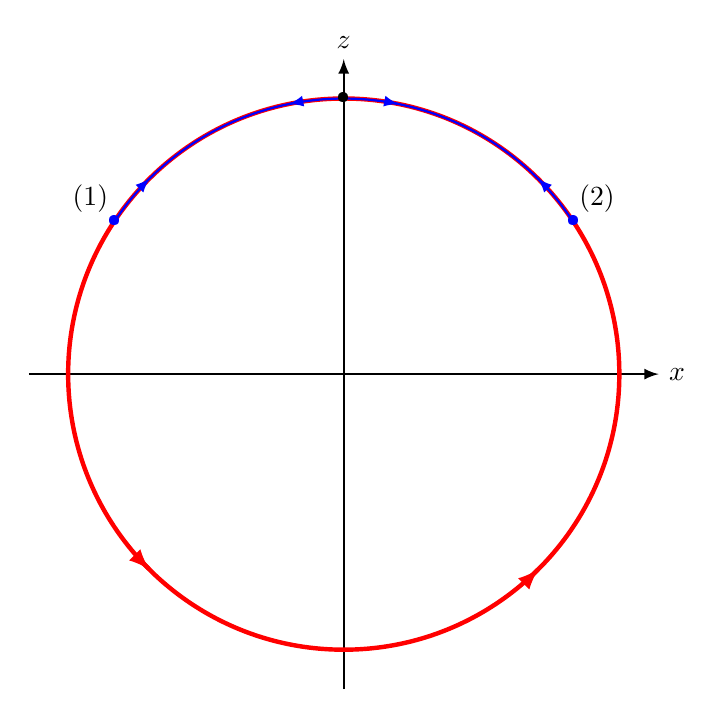
\begin{tikzpicture}
\draw[-latex, thick] ( 0.0, -4) -- (0, 4) node[above]{$z$};
\draw[-latex, thick] (-4,  0) -- (4, 0) node[right]{$x$};

\draw[red, ultra thick] (3.5, 0) arc (0:360:3.5);
\draw[-latex, red, ultra thick] (2.4648737348, -2.4848737348) -- (2.4748737348, - 2.4748737348);
\draw[-latex, red, ultra thick] (-2.4748737348, -2.4748737348) -- (-2.4648737348, -2.4848737348);

\draw[domain=33.540844097:146.459155903,smooth,variable=\x,blue, thick] plot ({3.5 * cos(\x)},{3.5 * sin(\x)});
\draw[-latex, blue, thick] (0.6853426578, 3.4322601227) -- (0.6953426578, 3.4302330223);
\draw[-latex, blue, thick] (2.4748737348,  2.4748737348) -- (2.4648737348, 2.4848737348);
\draw[-latex, blue, thick] (-0.6853426578, 3.4322601227) -- (-0.6953426578, 3.4302330223);
\draw[-latex, blue, thick] (-2.4748737348,  2.4748737348) -- (-2.4648737348, 2.4848737348);

%nodes:
\node[black] at (0, 3.5) {\textbullet};
\node[blue] at (-2.9172225397, 1.9338595227) {\textbullet};
\node[black] at (-2.9172225397 - 0.3, 1.9338595227 + 0.3) {(1)};
\node[blue] at (2.9172225397, 1.9338595227) {\textbullet};
\node[black] at (2.9172225397 + 0.3, 1.9338595227 + 0.3) {(2)};


\end{tikzpicture}
\caption{$\hat{h}(k)$ plotted as function of $k$. The angle with respect to the $z$ axis is given by $\tan(\theta_k) = \Delta^{11}_k/\varepsilon_k$.  In blue: $\mu > 0$. The blue curve starts on the north pole, at the black dot. It then goes counterclockwise until it reaches the point (1). It turns around, goes clockwise until it reaches (2). Finally it returns to the north pole. The total winding number is $w = 0$. In red: $\mu < 0$. The red curve starts and ends at the north pole, at the black dot. It goes counterclockwise around 0. The total winding number is $w = -1$. }
\label{fig.hhatplot}
\end{figure}

We now return to the system at hand. We have $h_z(k) = \varepsilon_k$ and $h_x(k) = \Delta^{11}_k$. If we let $\theta_k$ denote the angle of $\hat{h}(k)$ with the $z$-axis, the winding number is:
\begin{equation}
w = \frac{1}{2\pi}\oint d\theta_k.
\label{eq.definition.windingnumber}
\end{equation} 
The angle $\theta_k$ is given by: $\tan(\theta_k) = \frac{h_x(k)}{h_z(k)} = \frac{\Delta^{11}_k}{\varepsilon_k}$. In turn $\theta_k(c) = \arctan\left(\frac{\Delta^{11}_k}{\varepsilon_k}\right) + c$ for some constant $c$. Calculating $d\theta_k = dk \cdot \partial_k \theta_k$ then gives:
\begin{equation}
w = \frac{1}{2\pi}\int dk \frac{\varepsilon_k\partial_k\Delta^{11}_k - \Delta^{11}_k\partial_k\varepsilon_k}{\varepsilon^2_k + (\Delta^{11}_k)^2} = 2\text{CS}_{1,1}(\Delta^{12}_k = 0). \nonumber
\end{equation} 
Hence, we see that for the separated wires, the Chern-Simons invariant for wire 1 is simply twice the winding of $\hat{h}$ around $\mathbf{h} = 0$. We can hereby very directly understand, why the Chern-Simons invariant is in fact a topological invariant, at least for the separated wires. We have depicted the winding of $\hat{h}(k)$ in figure \ref{fig.hhatplot}. Here we assume, that $\Delta^{11}_k$ is negative for $k < 0$ and positive for $k > 0$. 

\subsection{Edge states: approximate solutions}
\label{subsec.2wiresedgestates}
In this section we come with an approximate analytical solution for the edge states for the separated wires. This is done for a later discussion on their properties. The analysis is largely based on \cite[pp. 196-198]{BernevigTITSC}. 

\begin{figure}
\center
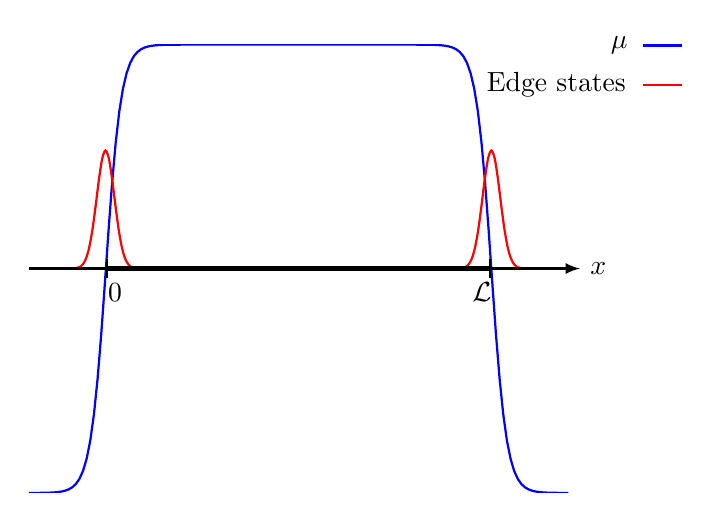
\begin{tikzpicture}
\begin{axis}[samples=150, xtick=\empty, ytick=\empty, axis line style={draw=none}, 
    xmin=-1, xmax=6,
    ymin = -1/2, ymax = 1/2,
    axis lines=center,
    domain=-1:6,
    ]

    \addplot [mark=none,draw=blue, thick] {1/2 * (tanh(5 * \x) - tanh(5 * (\x - 5) ) - 1)};
\end{axis}


\draw[scale=0.5,domain=-1:1,smooth,variable=\x,red, thick] plot ({\x + 0.975 * 2},{ 2 * 2.85 + 3 * exp{- 10 * \x*\x}});
\draw[scale=0.5,domain=-1:1,smooth,variable=\x,red, thick] plot ({\x + 5.875 * 2},{ 2 * 2.85 + 3 * exp{- 10 * \x*\x}});

\node at (0.975 + 0.12, 2.85 - 0.3) {$0$};
\node at (5.875-0.12, 2.85 - 0.3) {$\mathcal{L}$};
\draw[-latex, thick ] (0,2.85) -- (7,2.85) node[right]{$x$};
\draw[-, ultra thick ] (0.975,2.85) -- (5.875,2.85);
\draw[|-, thick ] (0.975,2.85) -- (1,2.85);
\draw[-, ultra thick ] (0.975,2.85) -- (5.875,2.85);
\draw[-|, thick ] (5.7,2.85) -- (5.875,2.85);

\coordinate (a) at (7.8, 5.682);
\coordinate (anode) at (7.5, 5.682);
\coordinate (b) at (8.3, 5.682);
\coordinate (c) at (7.8, 5.182);
\coordinate (d) at (8.3, 5.182);
\coordinate (cnode) at (6.7, 5.182);

\draw[-, thick, blue] (a) -- (b);
\node at (anode) {$\mu$}; 
\draw[-, thick, red] (c) -- (d);
\node at (cnode) {Edge states}; 
\end{tikzpicture}
\caption{Red: Edge states. Blue: chemical potential $\mu = \mu(x)$. Due to the spatial variation of the chemical potential the fermions are confined to the interval between $x = 0$ and $x = \mathcal{L}$. The separated wires are topological for $\mu > 0$. For $\mu < 0$ they are trivial. Hence, edge states form around $\mu = 0$ at $x = 0$ and $x = \mathcal{L}$. }
\label{fig.edgestatesmux}
\end{figure}

We would like to describe the Hamiltonian in real space, because we now ask whether certain states exist at the ends of the wires. To do this we define the operator $\Delta^{11}(p)$ as a function of the momentum operator $p = -i\partial_x$ in the following manner:
\begin{equation}
\Delta^{11}(p)\text{e}^{ikx} = \Delta^{11}_k\text{e}^{ikx}.
\label{eq.Deltapdef}
\end{equation}
Hence, we replace the variable dependency of $k$ in $\Delta^{11}_k$ with an operator dependency on $p$ in $\Delta^{11}(p)$. With this definition we get the Hamiltonian in real space:
\begin{equation}
H_{FF} = \frac{1}{2}\int dx\; \Psi^\dagger_{F}(x) \mathcal{H}_{FF}(x) \Psi_{F}(x), \hspace{0.5cm} \Psi_{F}(x) = \begin{bmatrix} \psi_{1,F}(x) & \psi^\dagger_{1,F}(x) & \psi_{2,F}(x) & \psi^\dagger_{2,F}(x)\end{bmatrix}^t
\label{eq.2wiresMFHamiltonianrealspace}
\end{equation}
With the real space Hamiltonian kernel:
\begin{equation}
\mathcal{H}_{FF}(x) = \begin{bmatrix} 
\frac{p^2}{2m_F} - \mu & \Delta^{11}(p) & 0 & 0 \\
\Delta^{11}(p) & -\left(\frac{p^2}{2m_F} - \mu \right) & 0 & 0 \\
0 & 0 & \frac{p^2}{2m_F} - \mu & -\Delta^{11}(p) \\
0 & 0 & -\Delta^{11}(p) & -\left(\frac{p^2}{2m_F} - \mu \right)
\end{bmatrix}.
\label{eq.2wiresMFHamiltonianrealspacefirstquantization}
\end{equation}
For the sake of clarity let us see how e.g. the term $\Delta^{11}_kc_{1,-k}c_{1,k}$ appears from this expression:
\begin{align}
\int dx \; \psi_{1,F}(x) \Delta^{11}(p) \psi_{1,F}(x) &= \frac{1}{\mathcal{L}}\sum_{k,q}c_{1,k} c_{1,q}\int dx \; \text{e}^{ikx}\Delta^{11}(p)\text{e}^{iqx} = \frac{1}{\mathcal{L}}\sum_{k,q}\Delta^{11}_qc_{1,k}c_{1,q}\int dx \; \text{e}^{i(k + q)x} \nonumber \\
&= \sum_{k}\Delta^{11}_kc_{1,-k}c_{1,k}, \nonumber 
\end{align}
since $\int dx\; \text{e}^{i(k + q)x} =\mathcal{L} \delta_{k,-q} $. Here we use the Fourier decomposition $\psi_{1,F}(x) = \frac{1}{\sqrt{L}}\sum_k\text{e}^{ikx}c_{1,k}$. Now we form junctions of topogically distinct phases by changing the sign of $\mu$ at $x = 0$ and $x = \mathcal{L}$. Hence, we let $\mu = \mu(x)$ as shown in figure \ref{fig.edgestatesmux}. Due to the spatial variation of the chemical potential the fermions are confined to the wire between $x = 0$ and $x = \mathcal{L}$. In first quantization we find solutions by solving $\mathcal{H}(x)\psi(x) = E\psi(x)$. The edge states are zero energy modes, so we solve for $E = 0$. We assume, that $\mu(x)$ varies slowly over the interparticle length scale $1/k_F$. When this is fulfilled the solution $\psi(x)$ will also vary slowly and hence the curvature of $\psi(x)$ proportional to $p^2\psi(x)$ is negligible. This means, that to a good approximation we only keep the operator $p$ up to first order. In the numerical analysis we will see, that $\Delta^{11}_k$ is linear in $k$ for $k/k_F \ll 1$. This means, that $\Delta^{11}(p)$ is linear in $p$, when $p/k_F$ used on a state is small. Hence, we ignore $p^2/2m_F$ and let $\Delta^{11}(p) = \Delta^{11} \cdot \tilde{p}$, with $\Delta^{11} = k_F\left.\frac{\partial \Delta^{11}_k}{\partial k}\right|_{k=0}$ and $\tilde{p} = p/k_F$. We assume $\Delta^{11} > 0$. We take the ansatz:
\begin{equation}
\psi^{i}_1(x) = \exp\left(-\frac{k_F}{\Delta^{11}}\int_{0}^{x} dx'\; \mu(x') \right)\mathbf{u}^{i}_{1}, \hspace{0.5cm} \psi^{i}_2(x) = \exp\left(+\frac{k_F}{\Delta^{11}}\int_{\mathcal{L}}^{x} dx'\; \mu(x') \right)\mathbf{u}^{i}_{2}, \nonumber
\end{equation}  
The superscript ${}^i$ refers to the wire, the subscript ${}_j$ to which end the wave function is located. Since $\Delta^{11}$ is in units of energy the exponents are unitless. Since $\Delta^{11} > 0$, we see that these states are exponentially localized at the edges. From this we get eigenvalue equations for $\mathbf{u}^{i}_{j}$. Defining $g_1(x) = \frac{1}{N}\text{e}^{-\frac{k_F}{\Delta^{11}}\int_{0}^{x} dx' \mu(x')}$, $g_2(x) = \frac{1}{N}\text{e}^{+\frac{k_F}{\Delta^{11}}\int_{\mathcal{L}}^{x} dx' \mu(x')}$ and $N^2 = \int dx |g_j(x)|^2$ a normalization constant we hereby get the approximate solutions:
\begin{align}
\psi^1_1(x) &= g_1(x)\frac{\text{e}^{+i\pi/4}}{\sqrt{2}}\begin{bmatrix} 1 & -i & 0 & 0 \end{bmatrix}^t , \hspace{0.5cm} \psi^1_2(x) = g_2(x)\frac{\text{e}^{-i\pi/4}}{\sqrt{2}}\begin{bmatrix} 1 & +i & 0 & 0 \end{bmatrix}^t, \nonumber \\
\psi^2_1(x) &= g_1(x)\frac{\text{e}^{-i\pi/4}}{\sqrt{2}}\begin{bmatrix} 0 & 0 & 1 & +i \end{bmatrix}^t , \hspace{0.5cm} \psi^2_2(x) = g_2(x)\frac{\text{e}^{+i\pi/4}}{\sqrt{2}}\begin{bmatrix} 0 & 0 & 1 & -i \end{bmatrix}^t.
\end{align}
From equation \eqref{eq.2wiresTminuswireexchangefirstquantization} we have, that the time reversal operator that squares to minus the identity is given by: $\mathcal{T}_- = i\sigma_2\otimes\tau_0 \cdot K$. We hereby get: $\mathcal{T}_-\psi^1_1(x) = -\psi^2_1(x), \mathcal{T}_-\psi^1_2(x) = -\psi^2_2(x)$. The edge states at the same end in each wire are therefore Kramers partners. This is crucial for the following analysis. For sake of completeness let us write up the second quantized version of the four states. The eigenstates define the diagonalisation matrix $U(x) = \begin{bmatrix} \psi^{1}_{1}(x) & \psi^{1}_{2}(x) & \psi^{2}_{1}(x) & \psi^{2}_{2}(x) \end{bmatrix}$. This has the unitarity property, that $\int dx \; U^\dagger(x) U(x) = \mathbb{I}$. We then let the operators $\gamma^{j}_{0,1}, \gamma^{j}_{0,2}$ for wire $j$ be given by:
\begin{equation}
\begin{bmatrix} \psi_{1,F}(x) \\ \psi_{1,F}^\dagger(x) \\ \psi_{2,F}(x) \\ \psi_{2,F}^\dagger(x) \end{bmatrix} = U(x) \begin{bmatrix} \gamma^{1}_{0,1} \\ \gamma^{1}_{0,2} \\ \gamma^{2}_{0,1} \\ \gamma^{2}_{0,2} \end{bmatrix} \Rightarrow \begin{bmatrix} \gamma^{1}_{0,1} \\ \gamma^{1}_{0,2} \\ \gamma^{2}_{0,1} \\ \gamma^{2}_{0,2} \end{bmatrix} = \int dx \; U^\dagger(x) \begin{bmatrix} \psi_{1,F}(x) \\ \psi_{1,F}^\dagger(x) \\ \psi_{2,F}(x) \\ \psi_{2,F}^\dagger(x) \end{bmatrix}.
\label{eq.Majoranaedgemodedef} 
\end{equation} 
Written out these operators are: 
\begin{align}
\gamma^1_{0,1} &= \int dx \; g_1(x)\frac{\text{e}^{-i\pi/4}}{\sqrt{2}}(\psi_{1,F}(x) + i\psi^\dagger_{1,F}(x)), \hspace{0.5cm} \gamma^1_{0,2} = \int dx \; g_2(x)\frac{\text{e}^{+i\pi/4}}{\sqrt{2}}(\psi_{1,F}(x) - i\psi^\dagger_{1,F}(x)), \nonumber \\
\gamma^2_{0,1} &= \int dx \; g_1(x)\frac{\text{e}^{+i\pi/4}}{\sqrt{2}}(\psi_{2,F}(x) - i\psi^\dagger_{2,F}(x)), \hspace{0.5cm} \gamma^2_{0,2} = \int dx \; g_2(x)\frac{\text{e}^{-i\pi/4}}{\sqrt{2}}(\psi_{2,F}(x) + i \psi^\dagger_{2,F}(x)). \nonumber 
\end{align}
In this manner $\psi^{i}_{j}(x)$ and $\gamma^{i}_{0,j}\ket{\text{S}}_0$ are equivalent. These operators are special in the sense, that they are their own antiparticle: $\left(\gamma^{i}_{0,j}\right)^\dagger = \gamma_{0,j}$.\footnote{This also illuminates why we chose the rather arbitrary phase factors $\text{e}^{\pm i\pi/4}$. Had we \textit{not} done this, there would be some phase difference between $\left(\gamma^{i}_{0,j}\right)^\dagger$ and $\gamma^{i}_{0,j}$.} Such a fermionic particle is called a Majorana mode in condensed matter physics. Besides being their own antiparticle, they have to obey the modified anticommutator relation:
\begin{equation}
\{\gamma^{i_1}_{0,j_1}, \gamma^{i_2}_{0,j_2} \} = \delta_{i_1,i_2}\delta_{j_1,j_2}. \nonumber
\end{equation}
This is explicitly verified to be the case for the above operators.\footnote{Often one also meets the requirement, that the anticommutator equals $2\delta_{i_1,i_2}\delta_{j_1,j_2}$. This is simply a matter of convention.} From this we can form regular but highly nonlocal fermionic operators: $d_j = \frac{1}{\sqrt{2}}(\gamma^{j}_{0,1} + i\gamma^{j}_{0,2})$. The key result of this section is thus, that $\ket{\text{S}}_0$ and $d_j^\dagger\ket{\text{S}}_0$ are degenerate ground states of the system. The topologically non-trivial state is therefore characterized by the presence of \textit{one} more particle than the trivial one, which is exponentially located on the edges.\footnote{In the literature one also meets the notion of a Majorana mode at each end, hence two in total. However, since $\gamma^\dagger_0\gamma_0 = \gamma_0^2 = \frac{1}{2}$ for Majorana operators, we cannot count them. Hence, the notion of a specific number of Majorana modes is undefined.}

In second quantization the above notion of Kramers partners is described by the fact, that: $T_-\gamma^1_{0,j}T_-^{-1} = \gamma^2_{0,j}$, simply because $\psi_{1,F}(x) \overset{T_-}{\to} \psi_{2,F}(x)$ and $T_-$ is antiunitary.

\section{Kramers degeneracy: protection of edge states}
\label{sec.2wireskramersdegeneracy}
In this section we show, that the interwire interaction protects the edge states as long as no interwire mean field has formed. We show, that this is because Kramers partners do not couple.

Consider a general system described by the Hamiltonian $H$. Assume, that this Hamiltonian is time reversal invariant, $[T, H] = 0$, and that $T^2 = -\mathbb{I}$. Let $\ket{\psi_1}$ and $\ket{\psi_2}$ be eigenstates to the Hamiltonian, with energy $E_1$ and $E_2$, and Kramers partners: $\ket{\psi_2} = T\ket{\psi_1}$. Since $[T, H] = 0$ the two states have the same energy: 
\begin{equation}
E_2\ket{\psi_2} = HT\ket{\psi_1} = TH\ket{\psi_1} = E_1\ket{\psi_2}. \nonumber
\end{equation}
So $E_2 = E_1$. Further, the states are orthogonal:
\begin{equation}
\braket{\psi_1|\psi_2} = \braket{T\psi_2|T\psi_1} = \braket{-\psi_1|\psi_2} = -\braket{\psi_1|\psi_2} \Rightarrow \braket{\psi_1|\psi_2} = 0. \nonumber  
\end{equation}
In the first equality we use, that we can flip the inner product by going to the time reversed states \cite[p. 274]{Sakurai}. In the second equality we use, that $T\ket{\psi_2} = -\ket{\psi_1}$, since $T^2 = -\mathbb{I}$. Hence, any energy state in a time reversal invariant system with $T^2 = -\mathbb{I}$ is twofold degenerate. This is Kramers degeneracy. Now let $H'$ be a perturbation to the Hamiltonian, which respects the time reversal symmetry: $[T, H'] = 0$. In degenerate perturbation theory we calculate the matrix with entries $W_{ij} = \bra{\psi_i}H'\ket{\psi_j}$. The eigenstates of $H$ remain good eigenstates if the states uncouple: $\bra{\psi_1}H'\ket{\psi_2} = 0$, so that $W_{ij}$ is diagonal. This is exactly the case for Kramers partners: 
\begin{equation}
\bra{\psi_1}H'\ket{\psi_2} = \bra{T\psi_2}TH'T^{-1}\ket{T\psi_1} = \bra{T\psi_2}H'\ket{T\psi_1} = -\bra{\psi_1}H'\ket{\psi_2} \Rightarrow \bra{\psi_1}H'\ket{\psi_2} = 0. \nonumber
\end{equation}
The first equality holds, since $H'$ is hermitian \cite[p. 274]{Sakurai}. 

Now what has this to do with the system at hand? We let $\ket{\psi_{i}^{j}} = \gamma_{i,0}^{j}\ket{\text{S}}_0$ for $i, j = 1, 2$. In this way, $\ket{\psi_{1}^1}$ is the edge state in wire 1 at end 1, $\ket{\psi_{2}^1}$ in wire 1 at end 2, and so forth. From above we know, that the edge states at end $i$, $\ket{\psi_{i}^1}$ and $\ket{\psi_{i}^2}$, are Kramers partners. If we can show, that the interwire interaction $H' = H^\text{int}_{FF,12}$ is time reversal invariant under $T_-$, then the above analysis shows that the edge states at the same end of the wire cannot couple. From equation \eqref{eq.Hint12realspace} we have:
\begin{equation}
H^\text{int}_{FF,12} = \int dx_1 dx_2 \psi^\dagger_{1,F}(x_1)\psi^\dagger_{2,F}(x_2) \tilde{V}_{\text{ind}}^{12}(x_1-x_2,0) \psi_{2,F}(x_2)\psi_{1,F}(x_1),
\end{equation}
with $\tilde{V}_{\text{ind}}^{12}(x_1-x_2,0)$ the zero frequency induced interaction in real space. Now $T_-\psi_{1,F}(x)T^{-1}_- = \psi_{2,F}(x)$ and $T_-\psi_{2,F}(x)T^{-1}_- = -\psi_{1,F}(x)$. Finally, $\tilde{V}_{\text{ind}}^{12}(x, 0)$ is real, so we get that $T_-H^\text{int}_{FF,12}T_-^{-1} = H^\text{int}_{FF,12}$. Hence, the edge states at the same end of the wire cannot couple. Further, the edge states at opposite ends of the wire are macroscopically separated. Therefore, these cannot couple either. In conclusion, the edge state in each wire is protected, as long as the interwire interaction is a perturbation to the system, which is to say no interwire mean field has formed.  

\section{Qualitative understanding of cross over}
\label{sec.2wirestransitionqualitative}
In this section we come with a qualitative analysis of how the cross over from $p$- to $s$-wave occures using the previous two sections. 

\textbf{Imaginary interwire pairing}: Assume that as the wires are brought closer together, the system chooses the interwire pairing to be \textit{imaginary}. Then the system \textit{breaks} the time reversal symmetry $T_-$. In this case there is no longer a Kramers degeneracy. As a consequence the edge states can couple and gap away. We can actually calculate by how much the edge states gap. In this connection we define the operator $\Delta^{12}(p)$ as: $\Delta^{12}(p)\text{e}^{ikx} = \Delta^{12}_k\text{e}^{ikx}$. Since $\Delta^{12}_k$ is even in $k$, there is no first order term in $k$. Hence for states with small curvatures like the edge states we can approximate $\Delta^{12}(p) = \Delta^{12}_{k=0}$. This means, that the perturbation in real space relevant for the edge states is:
\begin{equation}
\mathcal{H}'_{FF}(x) = \Delta^{12}_{k=0}\begin{bmatrix} 
0 & 0 &  0 & -i \\
0 & 0 & -i & 0 \\
0 & i & 0  & 0 \\
i & 0 & 0  & 0  \end{bmatrix}
\label{eq.interwirepairingrealspace}
\end{equation}
The edge states in wires 1 and 2 in first quantization are described by the wave functions $\psi^1_1, \psi^2_1, \psi^1_2, \psi^2_2$ found in subsection \ref{subsec.2wiresedgestates}. With this as an ordered basis we can calculate the perturbation matrix $W$ with entries $\bra{\psi^{i}_j}\mathcal{H}'\ket{\psi^{l}_k}$. We get:
\begin{equation}
W = \Delta^{12}_{k=0} \begin{bmatrix} 
0 & 0 & -i &  0 \\
0 & 0 &  0 & -i \\
i & 0 &  0 & 0 \\
0 & i &  0 & 0 \end{bmatrix} \nonumber
\end{equation}  
There are also couplings between the edge state at one end in wire 1 with the edge state at the other end in wire 2 and vice versa. This coupling is proportional to $\int dx \; g_1(x)g_2(x)$ and is therefore exponentially suppressed by the length of the wire. Hence, it is negligible for a macroscopic system. In this sense the only nonzero couplings are between the edge states at the same end in each wire. The shift in energies are the eigenvalues of $W$. These along with the corresponding perturbed wave functions are then given by:
\begin{align}
E &= +\Delta^{12}_{k=0}, \hspace{0.5cm} \frac{1}{\sqrt{2}}\left( \psi^1_j(x) + i\psi^2_j(x) \right), \nonumber \\
E &= -\Delta^{12}_{k=0}, \hspace{0.5cm} \frac{1}{\sqrt{2}}\left(\psi^1_j(x) - i\psi^2_j(x) \right),
\label{eq.perturbededgestates}
\end{align}
for the edge at $x = 0$ and $x = \mathcal{L}$ indicated by $j = 1$ and $j = 2$ respectively. Hence, the interwire pairing couples the two edge states in each wire around $x = 0$ and the two edge states around $x = \mathcal{L}$. This makes it explicit, how the states are gapped! This is the content of figure \ref{fig.2wiresedgestates} going from the top center to the middle left. 

\textbf{Real interwire pairing}: Assume that as the wires are brought closer together, the system chooses the interwire pairing to be \textit{real}. In this situation the system still respects the time reversal symmetry $T_-$. Kramers degeneracy is still present and therefore any energy state must be twofold degenerate. Further, since the system has a particle-hole symmetry the energy spectrum is symmetric around $E = 0$ (relative to the ground state). Therefore the zero energy edge states are locked as long as the bulk energy gap remains open. A direct calculation of the first order energy shift performed in the same way as in the above verifies this explicitly. The bulk energy dispersions in this situation are given by: $E^{\pm}_{F,k} = \sqrt{\varepsilon^2_k + (\Delta^{11}_k \pm \Delta^{12}_k)^2}$. The bulk gap will therefore eventually close as we bring the wires closer together. This happens exactly when $|\Delta^{12}_{k_0}| = |\Delta^{11}_{k_0}|$, where $\pm k_0$ are the Fermi points given by: $\varepsilon_{\pm k_0} = 0$. Hence, we expect a topological phase transition in this situation, with a topologically non-trivial system for $|\Delta^{12}_{k_0}| < |\Delta^{11}_{k_0}|$ and topologically trivial for $|\Delta^{12}_{k_0}| > |\Delta^{11}_{k_0}|$. This is the content of figure \ref{fig.2wiresedgestates} going from the top center to the middle and bottom right. 

\begin{figure}
\center
\begin{tikzpicture}
\draw[|-latex, thick] (0, 0) -- (0,  2) node[above]{$E$};
\draw[-, thick]   (0, 0) -- (0, -2);
\node at (-0.4, 0) {$0$};

\draw[-, dashed] (0, 1)--(2, 1);
\draw[-, thick] (-0.1, 1)--(0.1, 1);
\node at (-0.7,1) {$E_{F,k_0}$};

\draw[-, dashed] (0,    -1) -- (2,   -1);
\draw[-, thick]  (-0.1, -1) -- (0.1, -1);
\node at (-0.85,-1) {$-E_{F,k_0}$};

\draw[-, ultra thick] (1, 1)--(1, 2);
\draw[-, ultra thick] (1, -1)--(1, -2);
\node[red] at (1, 0) {\textbullet};

\draw[-, ultra thick] (2, 1)--(2, 2);
\draw[-, ultra thick] (2, -1)--(2, -2);
\node[blue] at (2, 0) {\textbullet};

\draw[-, dashed] (0,0.01) -- (2,0.01);

\node at (3, -1.9) {$0$};
\node at (5, -1.9) {$\mathcal{L}$};

\draw[scale=0.5,domain=-1:1,smooth,variable=\x,red] plot ({\x + 6},{ 2 * exp{- 15 * \x*\x} - 3});
\draw[scale=0.5,domain=-1:1,smooth,variable=\x,red] plot ({\x + 10},{ 2 * exp{- 15 * \x*\x} -3});
\draw[|-latex, thick ] (3,-1.5) -- (5.8,-1.5) node[right]{$x$};
\draw[-, ultra thick ] (3,-1.5) -- (5,-1.5);

\node at (3, 1.1) {$0$};
\node at (5, 1.1) {$\mathcal{L}$};

\draw[scale=0.5,domain=-1:1,smooth,variable=\x,blue] plot ({\x + 6},{ 2 * exp{- 15 * \x*\x} + 3});
\draw[scale=0.5,domain=-1:1,smooth,variable=\x,blue] plot ({\x + 10},{ 2 * exp{- 15 * \x*\x} + 3});

\draw[|-latex, thick ] (3,1.5) -- (5.8,1.5) node[right]{$x$};
\draw[-, ultra thick] (3, 1.5) -- (5, 1.5);

%\draw[-, dashed] (5.8, -1.5) -- (5.8, 1.5);
\node at (2.2, 2.8) {$\Delta^{12}_k = 0$};

%%%%%%%%%%%%%%%%%%%%%%%%%%%%%%%%%%%
\pgfmathsetmacro{\hmove}{-4}
\pgfmathsetmacro{\vmove}{-6}

\draw[|-latex, thick] (\hmove, \vmove) -- (\hmove,  2 + \vmove) node[above]{$E$};
\draw[-, thick]   (\hmove, \vmove) -- (\hmove, -2 + \vmove);
\node at (-0.4 + \hmove, 0 + \vmove) {$0$};

\draw[-, dashed] (0 + \hmove, 1 + \vmove)--(2 + \hmove, 1 + \vmove);
\draw[-, thick] (-0.1 + \hmove, 1 + \vmove)--(0.1 + \hmove, 1 + \vmove);
\node at (-0.7 + \hmove, 1 + \vmove) {$E_{F,k_0}$};

\draw[-, dashed] (0 + \hmove,    -1 + \vmove) -- (2 + \hmove,   -1 + \vmove);
\draw[-, thick]  (-0.1 + \hmove, -1 + \vmove) -- (0.1 + \hmove, -1 + \vmove);
\node at (-0.85 + \hmove,-1 + \vmove) {$-E_{F,k_0}$};

\draw[-, ultra thick] (1 + \hmove, 1 + \vmove)--(1 + \hmove, 2 + \vmove);
\draw[-, ultra thick] (1 + \hmove, -1 + \vmove)--(1 + \hmove, -2 + \vmove);

%gapped edge state:
\coordinate (edge1energy) at (1 + \hmove, 0.5 + \vmove);
\node[right=0.0cm of edge1energy] {$+\Delta^{12}_{k=0}$}; 
\draw[-latex, semithick] (1 + \hmove, 0 + \vmove)--(1 + \hmove, 0.5 + \vmove);
\node[red] at (edge1energy) {\textbullet};

\draw[-, ultra thick] (2 + \hmove, 1 + \vmove)--(2 + \hmove, 2 + \vmove);
\draw[-, ultra thick] (2 + \hmove, -1 + \vmove)--(2 + \hmove, -2 + \vmove);

%gapped edge state:
\coordinate (edge2energy) at (2 + \hmove, -0.5 + \vmove);
\node[right=0.0cm of edge2energy] {$-\Delta^{12}_{k=0}$}; 
\draw[-latex, semithick] (2 + \hmove, 0 + \vmove)--(2 + \hmove, -0.5 + \vmove);
\node[blue] at (edge2energy) {\textbullet};

\draw[-, dashed] (0 + \hmove,0.01 + \vmove) -- (2 + \hmove,0.01 + \vmove);

\node at (3 + \hmove, -1.4 + \vmove) {$0$};
\node at (5 + \hmove, -1.4 + \vmove) {$\mathcal{L}$};

\draw[|-latex, thick ] (3 + \hmove,-1.0 + \vmove) -- (5.8 + \hmove,-1.0 + \vmove) node[right]{$x$};
\draw[-, ultra thick ] (3 + \hmove,-1.0 + \vmove) -- (5 + \hmove,-1.0 + \vmove);

\node at (3 + \hmove, 0.6 + \vmove) {$0$};
\node at (5 + \hmove, 0.6 + \vmove) {$\mathcal{L}$};

\draw[|-latex, thick ] (3 + \hmove, 1.0 + \vmove) -- (5.8 + \hmove,1.0 + \vmove) node[right]{$x$};
\draw[-, ultra thick] (3 + \hmove, 1.0 + \vmove) -- (5 + \hmove, 1.0 + \vmove);

\node at (2.2 + \hmove, 2.8 + \vmove) {$\Delta^{12}_k \neq 0$, imaginary};

%%%%%%%%%%%%%%%%%%%%%%%%%%%%%%%%%%%
\pgfmathsetmacro{\hmove}{4}
\pgfmathsetmacro{\vmove}{-6}
\pgfmathsetmacro{\Eminchange}{0.4}

\draw[|-latex, thick] (\hmove, \vmove) -- (\hmove,  2 + \vmove) node[above]{$E$};
\draw[-, thick]   (\hmove, \vmove) -- (\hmove, -2 + \vmove);
\node at (-0.4 + \hmove, 0 + \vmove) {$0$};

\draw[-, dashed] (0 + \hmove, 1 - \Eminchange + \vmove)--(2 + \hmove, 1 - \Eminchange + \vmove);
\draw[-, thick] (-0.1 + \hmove, 1 - \Eminchange + \vmove)--(0.1 + \hmove, 1 - \Eminchange + \vmove);
\node at (-0.7 + \hmove, 1 - \Eminchange + \vmove) {$E_{F,k_0}$};

\draw[-, dashed] (0 + \hmove,    -1 + \Eminchange + \vmove) -- (2 + \hmove,   -1 + \Eminchange + \vmove);
\draw[-, thick]  (-0.1 + \hmove, -1 + \Eminchange + \vmove) -- (0.1 + \hmove, -1 + \Eminchange + \vmove);
\node at (-0.85 + \hmove, -1 + \Eminchange + \vmove) {$-E_{F,k_0}$};

\draw[-, ultra thick] (1 + \hmove, 1 - \Eminchange + \vmove)--(1 + \hmove, 2 + \vmove);
\draw[-, ultra thick] (1 + \hmove, -1 + \Eminchange + \vmove)--(1 + \hmove, -2 + \vmove);
\node[red] at (1 + \hmove, 0 + \vmove) {\textbullet};

\draw[-, ultra thick] (2 + \hmove, 1 - \Eminchange + \vmove)--(2 + \hmove, 2 + \vmove);
\draw[-, ultra thick] (2 + \hmove, -1 + \Eminchange + \vmove)--(2 + \hmove, -2 + \vmove);
\node[blue] at (2 + \hmove, 0 + \vmove) {\textbullet};

\draw[-, dashed] (0 + \hmove, 0.01 + \vmove) -- (2 + \hmove, 0.01 + \vmove);

\node at (3 + \hmove, -1.4 + \vmove) {$0$};
\node at (5 + \hmove, -1.4 + \vmove) {$\mathcal{L}$};

\draw[scale=0.5,domain=-1:1,smooth,variable=\x,red] plot ({\x + 6 + 2*\hmove},{ 2 * exp{- 15 * \x*\x} - 2.0 + 2*\vmove});
\draw[scale=0.5,domain=-1:1,smooth,variable=\x,blue] plot ({\x + 10 + 2*\hmove},{ 2 * exp{- 15 * \x*\x} -2.0 + 2*\vmove});
\draw[|-latex, thick ] (3 + \hmove,-1.0 + \vmove) -- (5.8 + \hmove,-1.0 + \vmove) node[right]{$x$};
\draw[-, ultra thick ] (3 + \hmove,-1.0 + \vmove) -- (5 + \hmove,-1.0 + \vmove);

\node at (3 + \hmove, 0.6 + \vmove) {$0$};
\node at (5 + \hmove, 0.6 + \vmove) {$\mathcal{L}$};

\draw[scale=0.5,domain=-1:1,smooth,variable=\x,red] plot ({\x + 6  + 2*\hmove},{ 2 * exp{- 15 * \x*\x} + 2.0 + 2*\vmove});
\draw[scale=0.5,domain=-1:1,smooth,variable=\x,blue] plot ({\x + 10 + 2*\hmove},{ 2 * exp{- 15 * \x*\x} + 2.0 + 2*\vmove});

\draw[|-latex, thick ] (3 + \hmove,1.0 + \vmove) -- (5.8 + \hmove,1.0 + \vmove) node[right]{$x$};
\draw[-, ultra thick] (3 + \hmove, 1.0 + \vmove) -- (5 + \hmove, 1.0 + \vmove);

\node at (2.2 + \hmove, 2.8 + \vmove) {$|\Delta^{12}_{k_0}| < |\Delta^{11}_{k_0}|$, real};

%squezzing of gap:
\draw[-latex, semithick] (0.5 + \hmove, 1  + \vmove)--(0.5 + \hmove, 1 - \Eminchange + \vmove);
\draw[-latex, semithick] (0.5 + \hmove, -1 + \vmove)--(0.5 + \hmove, -1 + \Eminchange + \vmove);

%%%%%%%%%%%%%%%%%%%%%%%%%%%%%%%%%%%
\pgfmathsetmacro{\hmove}{4}
\pgfmathsetmacro{\vmove}{-12}
\pgfmathsetmacro{\Eminchange}{0.4}

\draw[|-latex, thick] (\hmove, \vmove) -- (\hmove,  2 + \vmove) node[above]{$E$};
\draw[-, thick]   (\hmove, \vmove) -- (\hmove, -2 + \vmove);
\node at (-0.4 + \hmove, 0 + \vmove) {$0$};

\draw[-, dashed] (0 + \hmove, 1 - \Eminchange + \vmove)--(2 + \hmove, 1 - \Eminchange + \vmove);
\draw[-, thick] (-0.1 + \hmove, 1 - \Eminchange + \vmove)--(0.1 + \hmove, 1 - \Eminchange + \vmove);
\node at (-0.7 + \hmove, 1 - \Eminchange + \vmove) {$E_{F,k_0}$};

\draw[-, dashed] (0 + \hmove,    -1 + \Eminchange + \vmove) -- (2 + \hmove,   -1 + \Eminchange + \vmove);
\draw[-, thick]  (-0.1 + \hmove, -1 + \Eminchange + \vmove) -- (0.1 + \hmove, -1 + \Eminchange + \vmove);
\node at (-0.85 + \hmove, -1 + \Eminchange + \vmove) {$-E_{F,k_0}$};

\draw[-, ultra thick] (1 + \hmove, 1 - \Eminchange + \vmove)--(1 + \hmove, 2 + \vmove);
\draw[-, ultra thick] (1 + \hmove, -1 + \Eminchange + \vmove)--(1 + \hmove, -2 + \vmove);
%\node[red] at (1 + \hmove, 0 + \vmove) {\textbullet};

\draw[-, ultra thick] (2 + \hmove, 1 - \Eminchange + \vmove)--(2 + \hmove, 2 + \vmove);
\draw[-, ultra thick] (2 + \hmove, -1 + \Eminchange + \vmove)--(2 + \hmove, -2 + \vmove);
%\node[blue] at (2 + \hmove, 0 + \vmove) {\textbullet};

\draw[-, dashed] (0 + \hmove, 0.01 + \vmove) -- (2 + \hmove, 0.01 + \vmove);

\node at (3 + \hmove, -0.9 + \vmove) {$0$};
\node at (5 + \hmove, -0.9 + \vmove) {$\mathcal{L}$};

\draw[|-latex, thick ] (3 + \hmove,-0.5 + \vmove) -- (5.8 + \hmove,-0.5 + \vmove) node[right]{$x$};
\draw[-, ultra thick ] (3 + \hmove,-0.5 + \vmove) -- (5 + \hmove,  -0.5 + \vmove);

\node at (3 + \hmove, 0.1 + \vmove) {$0$};
\node at (5 + \hmove, 0.1 + \vmove) {$\mathcal{L}$};

\draw[|-latex, thick ] (3 + \hmove,0.5 + \vmove) -- (5.8 + \hmove,0.5 + \vmove) node[right]{$x$};
\draw[-, ultra thick] (3 + \hmove, 0.5 + \vmove) -- (5 + \hmove,  0.5 + \vmove);

\node at (2.2 + \hmove, 2.8 + \vmove) {$|\Delta^{12}_{k_0}| > |\Delta^{11}_{k_0}|$, real};

%squezzing of gap:
\draw[-latex, semithick] (0.5 + \hmove, 1 - \Eminchange + \vmove)--(0.5 + \hmove, 1  + \vmove);
\draw[-latex, semithick] (0.5 + \hmove, -1 + \Eminchange + \vmove)--(0.5 + \hmove, -1 + \vmove);

\end{tikzpicture}
\caption{\textbf{Top centered}: for $\Delta^{12}_k=0$ we have two copies of the single wire system with the interwire interaction as a perturbation. There are two symmetry-protected edge states, one at each wire and two energy dispersions mirrored in $E = 0$. This is indicated with red and blue dots. $k_0$ is defined by: $0 = \varepsilon_{k_0} = \frac{k^2_0}{2m_F} - \mu$. \textbf{Middle left}: If the system chooses an imaginary interwire pairing the system breaks the $T^2 = -\mathbb{I}$ symmetry. The edge states are therefore no longer protected at $E = 0$, and the edge states are gapped by $2\Delta^{12}_{k=0}$. \textbf{Middle and bottom right}: If the system chooses a real interwire pairing the system still respects the $T^2 = -\mathbb{I}$ symmetry. \textbf{Middle right}: Before an energy gap closing the edge states are still protected. Due to the interwire pairing the two edge states are located equally on each wire in opposite ends. Hence, the colours of the wave functions. The gap is closing; this is indicated by the arrows squezzing the gap. 
\textbf{Bottom right}: After the gap closing the edge states are gone. The system is topologically trivial. The gap is opening again indicated by the arrows.}
\label{fig.2wiresedgestates}
\end{figure}

It turns out that we can find approximate eigenstates for $\Delta^{12}_{k=0} \ll \Delta^{11}$. We take the ansatz $\psi_j^{\pm}(x) = g_j^{\pm}(x)\cdot \mathbf{u}^{\pm}_j$ for four component vectors $\mathbf{u}^{\pm}_j$. Further $g_1^{\pm}(x) = \frac{1}{N}\text{e}^{-\frac{k_F}{\Delta^{11}}\int_0^x dx' \; \left[\mu(x') \pm i\Delta^{12}_{k=0}\right] }$ and $g_2^{\pm}(x) = \frac{1}{N}\text{e}^{+\frac{k_F}{\Delta^{11}}\int_{\mathcal{L}}^x dx' \; \left[\mu(x') \pm i\Delta^{12}_{k=0}\right] }$. We then seach for solutions to $(\mathcal{H}_{FF}(x) + \mathcal{H}'_{FF}(x))\psi_j^{\pm}(x) = 0$, only keeping $p$ up to first order. The first and second derivative ($l = 1$ and $l = 2$) has a term proportional to $\left(\frac{\Delta^{12}_{k=0}}{\Delta^{11}}\right)^l\psi_j^{\pm}(x)$. Since we only keep $p$ up to first order, the second derivative must be small with respect to the first one. It is then clear, that $\left(\frac{\Delta^{12}_{k=0}}{\Delta^{11}}\right)^2 \ll \frac{\Delta^{12}_{k=0}}{\Delta^{11}}$ is required. In turn $\Delta^{12}_{k=0} \ll \Delta^{11}$. As $\Delta^{12}_{k=0}$ comes closer to $\Delta^{11}$ we must add higher order terms in $p$ to get accurate results. With the above ansatz we get the following solutions in the $\Delta^{12}_{k=0} \ll \Delta^{11}$ regime:
\begin{align}
\psi_1^{+}(x) &= \frac{g_1^{+}(x)}{2}\begin{bmatrix} 1 & -i & 1 & i \end{bmatrix}^t, \hspace{0.5cm} \psi_1^{-}(x) = \frac{g_1^{-}(x)}{2}\begin{bmatrix} i & 1 & -i & 1 \end{bmatrix}^t, \nonumber \\
\psi_2^{+}(x) &= \frac{g_2^{+}(x)}{2}\begin{bmatrix} 1 & i & -1 & i \end{bmatrix}^t, \hspace{0.5cm} \psi_2^{-}(x) = \frac{g_2^{-}(x)}{2}\begin{bmatrix} -i & 1 & -i & -1 \end{bmatrix}^t.
\label{eq.zeromodesDelta12real}
\end{align}
The two first components of these vectors are the parts of the wave functions in wire 1, the last two components the parts of the wave functions in wire 2. Since the norms of these components are the same, the effect of the interwire pairing is, that the new edge states are localised with even probability in each wire, one around $x = 0$ and one around $x = \mathcal{L}$. This is indicated in the middle right of figure \ref{fig.2wiresedgestates} by the colours of the wave functions. Further, to lowest order in $\Delta^{12}_{k = 0}/\Delta^{11}$ the edge state wave functions simply acquire a space dependent phase proportional to $\Delta^{12}_{k=0}$.  

